\documentclass[aspectratio=169,usenames,dvipsnames]{beamer}
\beamertemplatenavigationsymbolsempty
% \documentclass{beamer}

% UNCOMMENT FOR HANDOUTS
% \usepackage{pgfpages}
% \pgfpagesuselayout{2 on 1}[landscape,letterpaper,border shrink=5mm]
% \setbeameroption{show notes}

\mode<presentation>
\usetheme{Boadilla}
\usecolortheme{spruce}
\usepackage{../../LizStyle,ulem}
\usepackage{color}
\usepackage[color,matrix,arrow]{xy}
% \input xy
% \xyoption{all}
\usepackage{tikz}
\usepackage{tikz-cd}
\tikzset{commutative diagrams/diagrams={ampersand replacement=\&}}

\AtBeginSection{\frame{\sectionpage}}


% ==========Command for putting comments and removing them=======
% Visible:
\newcommand{\InstructorNotes}[1]{\textit{\color{orange}#1}}
\newcommand{\InstructorList}[1]{
\begin{itemize}
	\color{orange}
	#1
\end{itemize}
}
% Removed:
\renewcommand{\InstructorNotes}[1]{}
\renewcommand{\InstructorList}[1]{}


\newcommand{\bvfill}{\vskip0pt plus 1filll}

\usepackage{multimedia}
\usepackage{graphbox}

% \usepackage{algpseudocode}


\newcommand{\Reeb}{\textbf{Reeb}}
\newcommand{\Rtopc}{\textbf{Rtopc}}
% \newcommand{\RR}{\mathcal{R}}

\newcommand{\Set}{\textbf{Set}}
\newcommand{\Vect}{\textbf{Vect}}
\newcommand{\Top}{\textbf{Top}}
\newcommand{\Int}{\textbf{Int}}


\graphicspath{ {Figures/} {../../Figures/} }



\begin{document}
%\pdfoptionpdfminorversion 5
%\logo{\includegraphics[height=1.5cm]{dukeshield.pdf}}
\title[Review day]{Test 2 review day}
\subtitle{CMSE 381}
\date{Fri, March 14, 2025}



\institute[MSU-CMSE]{Michigan State University\\
			::\\
          Dept of Computational Mathematics, Science \& Engineering}
\author[Dr.~Zhang]{Prof.~Mengsen Zhang}

\begin{frame}
 \titlepage


\end{frame}
%--------------------------
\begin{frame}[c]{Announcements}

\begin{columns}

\column{.60\textwidth}
\centering

	Announcements: 
	\begin{itemize}
		\item midterm \# 2 on Monday
		\item HW 5 due Sunday (3/16)
	\end{itemize}
\end{columns}

\end{frame}
%--- Next Frame ---%
\begin{frame}[c]{Top questions submitted}

\begin{columns}
\column{.4\textwidth}
\centering
\begin{itemize}
	\item Compare different kinds of validation
	\item difference between lasso and ridge regression
	\item go through subset selection example again
	% \item Error rate (classification)
	% \item Bayes Classifier
	% \item $K$-NN classification
\end{itemize}
\column{.4\textwidth}
\centering

\end{columns}

\end{frame}
%--- Next Frame ---%

\begin{frame}[t]{Training error vs test error}
	\centering
	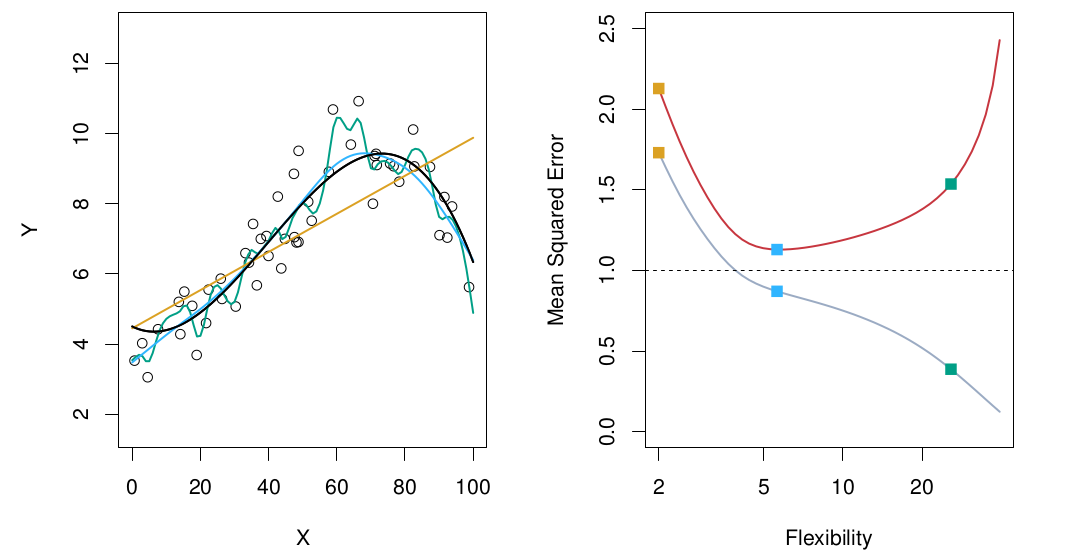
\includegraphics[width = .7\textwidth]{Fig2-9.png}


\tiny
	\InstructorList{
	\item Left: Black line is model for simulation of data
	\item Right side: training in blue/grey, testing in red
	\item Variance of $\e$ is dashed line
	\item Point out that training error goes down but test goes up (overfitting)
	\item Flexibility = degrees of freedom
	}
\end{frame}

%--- Next Frame ---%

\begin{frame}[t]{Approximations of Test Error}
	\begin{columns}
	\column{.3\textwidth}
	\centering
	\textbf{Validation Set}
	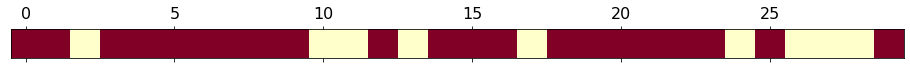
\includegraphics[width = \textwidth]{CV-subset0}
	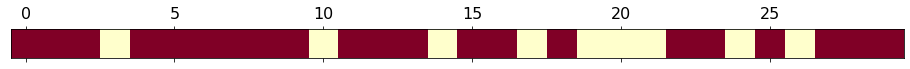
\includegraphics[width = \textwidth]{CV-subset1}
	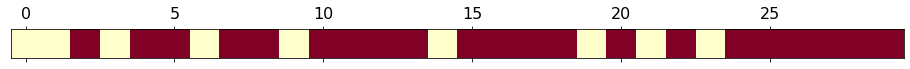
\includegraphics[width = \textwidth]{CV-subset2}
	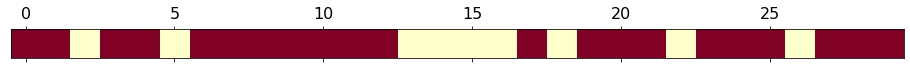
\includegraphics[width = \textwidth]{CV-subset3}
	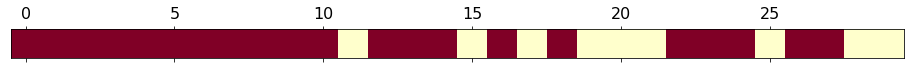
\includegraphics[width = \textwidth]{CV-subset4}
	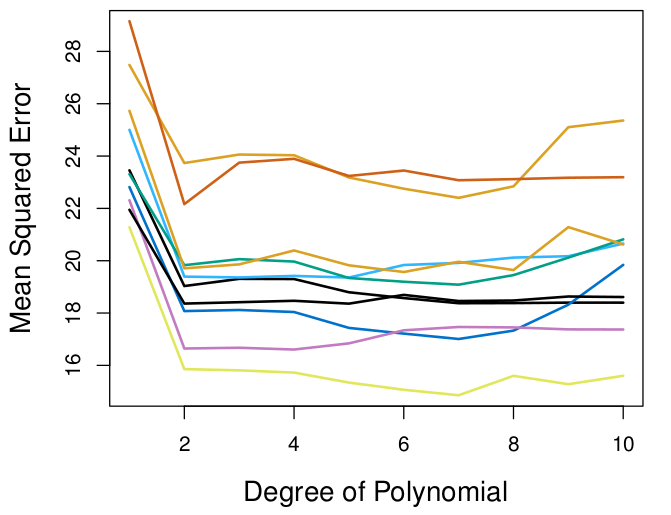
\includegraphics[width = .8\textwidth]{Fig5-2b}
	\column{.3\textwidth}
	\centering
	\textbf{LOOCV}
	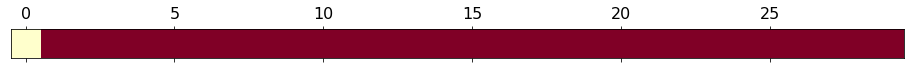
\includegraphics[width = \textwidth]{LOOCV-subset0.png}
	
\includegraphics[width = \textwidth]{LOOCV-subset1.png}
	
\includegraphics[width = \textwidth]{LOOCV-subset2.png}
	% 
\includegraphics[width = \textwidth]{LOOCV-subset3.png}
	% 
\includegraphics[width = \textwidth]{LOOCV-subset4.png}
	$\vdots$
	
\includegraphics[width = \textwidth]{LOOCV-subset29.png}
	
	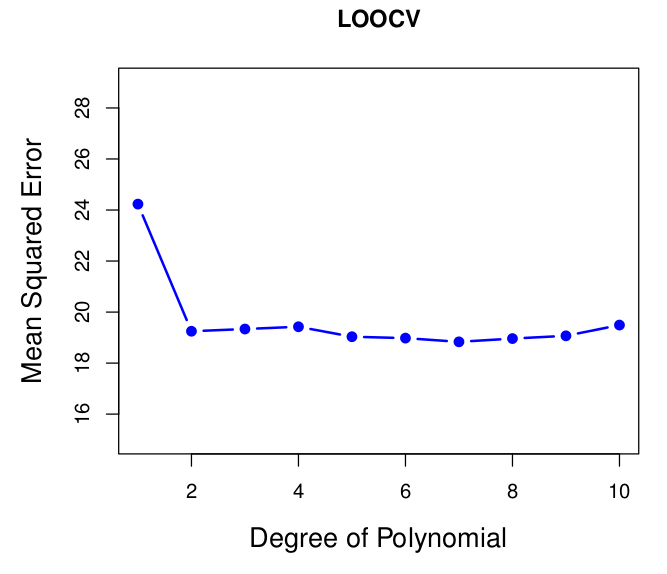
\includegraphics[width = .8\textwidth]{Fig5-4a}
	
	\column{.3\textwidth}
	\centering
	\textbf{K-fold CV}
	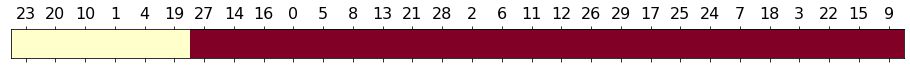
\includegraphics[width = \textwidth]{CV-Kfold-subset0}
	
\includegraphics[width = \textwidth]{CV-Kfold-subset1}
	
\includegraphics[width = \textwidth]{CV-Kfold-subset2}
	
\includegraphics[width = \textwidth]{CV-Kfold-subset3}
	
\includegraphics[width = \textwidth]{CV-Kfold-subset4}
	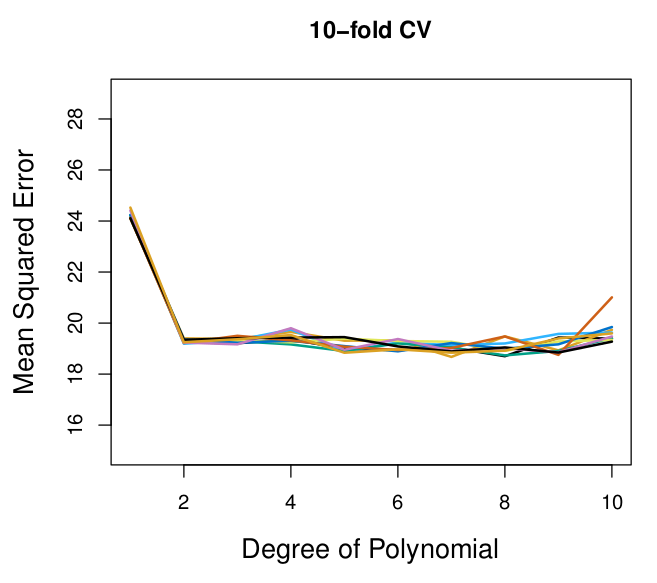
\includegraphics[width = .8\textwidth, align = c]{Fig5-4b}
	\end{columns}
	\end{frame}
	%--- Next Frame ---%
	\begin{frame}[t]{Validation set approach}

		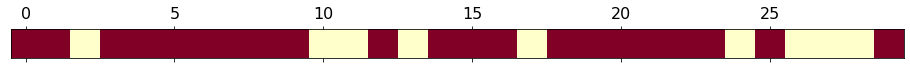
\includegraphics[width = \textwidth]{CV-subset0}
		
		\begin{columns}
		\column{.45\textwidth}
		\centering
		\begin{itemize}
			\item Divide randomly into two parts:
			\begin{itemize}
				\item Training set
				\item Validation/Hold-out/Testing set
			\end{itemize}
			\item Fit model on training set
			\item Use fitted model to predict response for observations in the test set
			\item Evaluate quality (e.g.~MSE)
		\end{itemize}
		\column{.45\textwidth}
		\centering
		\InstructorList{
		\item This example has 30 data points
		\item Keep out $30\% = 9 $ for testing in yellow
		\item We've done this in previous jupyter notebooks
		}
		\end{columns}
		
		\end{frame}
	
	%=====
\begin{frame}[c]{LOOCV}
	\centering
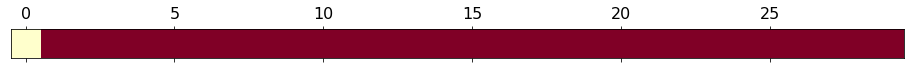
\includegraphics[width = \textwidth]{LOOCV-subset0.png}

\includegraphics[width = \textwidth]{LOOCV-subset1.png}

\includegraphics[width = \textwidth]{LOOCV-subset2.png}

\includegraphics[width = \textwidth]{LOOCV-subset3.png}

\includegraphics[width = \textwidth]{LOOCV-subset4.png}
$\vdots$

\includegraphics[width = \textwidth]{LOOCV-subset29.png}
\begin{columns}
\column{.45\textwidth}
\centering

\column{.45\textwidth}
\centering

\end{columns}

\end{frame}
%--- Next Frame ---%
\begin{frame}[c]{LOOCV in mathy words}

\begin{columns}
\column{.45\textwidth}
\centering
\begin{itemize}
	\item Remove $(x_1,y_1)$ for testing.
	\item Train the model on $n-1$ points: $\{(x_2,y_2), \cdots, (x_n,y_n)\}$
	\item Calculate $\mathrm{MSE}_1 = (y_1-\hat y_1)^2$
	\item[]
	\item Remove $(x_2,y_2)$ for testing.
	\item Train the model on $n-1$ points: $\{(x_1,y_1),(x_3,y_3), \cdots, (x_n,y_n)\}$
	\item Calculate $\mathrm{MSE}_2 = (y_2-\hat y_2)^2$
	\item []
	\item Rinse and repeat
\end{itemize}
\column{.45\textwidth}
\centering

Return the score:
\begin{equation*}
	CV_{(n)} = \frac{1}{n}\sum_{i=1}^n \mathrm{MSE}_i
\end{equation*}
\end{columns}

\end{frame}

	
	%--- Next Frame ---%
	\begin{frame}[c]{Definition of $k$-fold CV}
	
	\begin{columns}
	\column{.45\textwidth}
	\centering
	\begin{itemize}
		\item Randomly split data into $k$-groups (folds)
		\item Approximately equal sized. For the sake of notation, say each set has $\ell$ points
		\item []
		\item Remove $i$th fold $U_i$ and reserve for testing.
		\item Train the model on remaining points
		\item Calculate $\mathrm{MSE}_i = \frac{1}{\ell} \sum_{(x_j,y_j) \in U_i}(y_j-\hat y_j)^2$
		\item[]
		\item Rinse and repeat
	\end{itemize}
	\column{.45\textwidth}
	\centering
	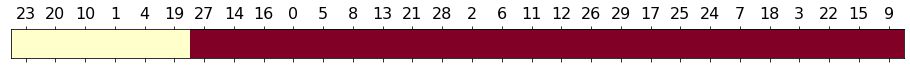
\includegraphics[width = \textwidth]{CV-Kfold-subset0}
	
\includegraphics[width = \textwidth]{CV-Kfold-subset1}
	
\includegraphics[width = \textwidth]{CV-Kfold-subset2}
	
\includegraphics[width = \textwidth]{CV-Kfold-subset3}
	
\includegraphics[width = \textwidth]{CV-Kfold-subset4}
	Return
	\begin{equation*}
		CV_{(k)} = \frac{1}{k} \sum_{i=1}^k \mathrm{MSE}_i
	\end{equation*}
	\end{columns}
	
	\end{frame}

%--- Next Frame ---%
\begin{frame}[c]{Setup: $k$-fold}

	\begin{columns}
	\column{.45\textwidth}
	\centering
	\begin{itemize}
		\item Randomly split data into $k$-groups (folds)
		\item Approximately equal sized. For the sake of notation, say each set has $\ell$ points
		\item []
		\item Remove $i$th fold $U_i$ and reserve for testing.
		\item Train the model on remaining points
		\item Calculate $\mathrm{Err}_i = \frac{1}{\ell} \sum_{(x_j,y_j) \in U_i}\mathrm{I}(y_j\neq\hat y_j)$
		\item[]
		\item Rinse and repeat
	\end{itemize}
	\column{.45\textwidth}
	\centering
	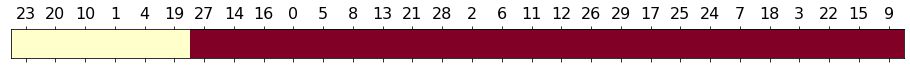
\includegraphics[width = \textwidth]{CV-Kfold-subset0}
	
\includegraphics[width = \textwidth]{CV-Kfold-subset1}
	
\includegraphics[width = \textwidth]{CV-Kfold-subset2}
	
\includegraphics[width = \textwidth]{CV-Kfold-subset3}
	
\includegraphics[width = \textwidth]{CV-Kfold-subset4}

	Return
	\begin{equation*}
		CV_{(k)} = \frac{1}{k} \sum_{i=1}^k \mathrm{Err}_i
	\end{equation*}
	\end{columns}

\end{frame}

%--- Next Frame ---%
\begin{frame}[t]{Ridge regression}

	\begin{columns}
	\column{.3\textwidth}
	\centering
	\textbf{Before:}
	\footnotesize
	\begin{equation*}
		RSS = \sum_{i=1}^n \left(y_i - \beta_0 - \sum_{j=1}^p \beta_j x_{ij}\right)^2
	\end{equation*}
	
	\column{.55\textwidth}
	\centering
	\textbf{After:}
	\begin{equation*}
		\sum_{i=1}^n \left(y_i - \beta_0 - \sum_{j=1}^p \beta_j x_{ij}\right)^2 + \lambda \sum_{j=1}^p \beta_j^2 = RSS + \lambda \sum_{j=1}^p \beta_j^2
	\end{equation*}
	
	\end{columns}
	
	\begin{columns}
	\column{.3\textwidth}
	\centering
	
	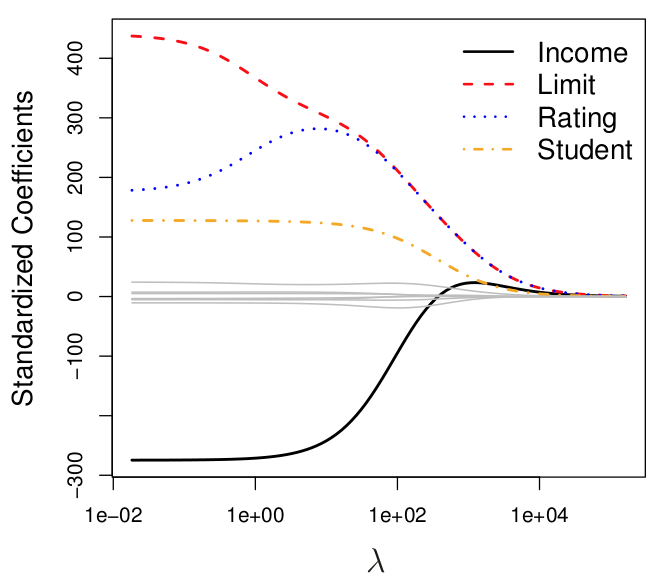
\includegraphics[width = \textwidth, align = c]{Fig6-4a}
	\column{.3\textwidth}
	\centering
	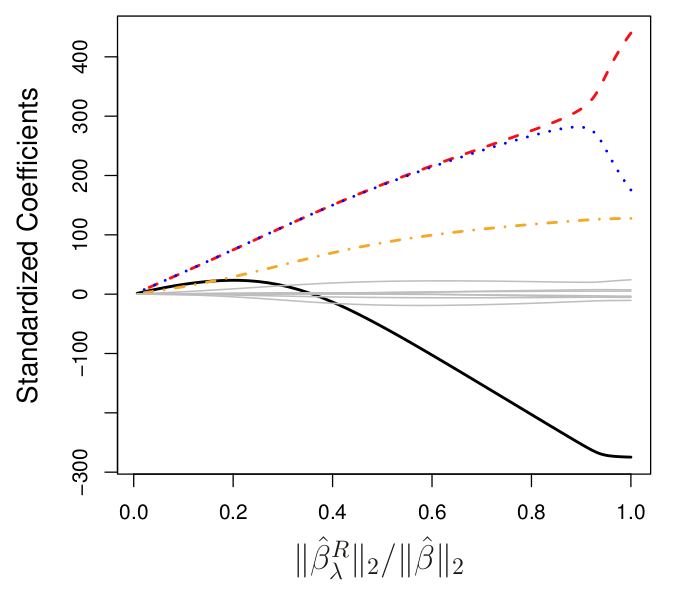
\includegraphics[width = \textwidth, align = c]{Fig6-4b}
	\end{columns}
	
	% \begin{columns}
	% \column{.45\textwidth}
	% \centering
	% \footnotesize
	% \InstructorList{
	% \item $\lambda \geq 0$ is a tuning paramter to figure out separately.
	% \item Second term is called ``shrinkage penalty''
	% \item $\lambda = 0$ means least squares estimate
	% }
	% \column{.45\textwidth}
	% \centering
	
	% \footnotesize
	% \InstructorList{
	% \item As $\lambda \to \infty$ impact of shrinkage penalty grows, ridge regression coeff will go towards 0
	% % \item note different set of estimates every time
	% \item Not applied to the intercept
	% \item call coefficients found by ridge regression $\hat \beta_\lambda^R = (\beta_{1,\lambda}^R, \cdots,\beta_{p,\lambda}^R \cdots )$
	% }
	% \end{columns}
	
	\end{frame}

%--- Next Frame ---%
\begin{frame}[t]{The lasso}

	\begin{columns}
	\column{.3\textwidth}
	\centering
	\textbf{Least Squares:}
	\footnotesize
	\begin{equation*}
		RSS = \sum_{i=1}^n \left(y_i - \beta_0 - \sum_{j=1}^p \beta_j x_{ij}\right)^2
	\end{equation*}
	
	\column{.55\textwidth}
	\centering
	\footnotesize
	\textbf{Ridge:}
	\begin{equation*}
		\sum_{i=1}^n \left(y_i - \beta_0 - \sum_{j=1}^p \beta_j x_{ij}\right)^2 + \lambda \sum_{j=1}^p \beta_j^2 = RSS + \lambda \sum_{j=1}^p \beta_j^2
	\end{equation*}
	
	\end{columns}
	\centering
	\qquad
	
	\textbf{The Lasso:}
	\begin{equation*}
		\sum_{i=1}^n \left(y_i - \beta_0 - \sum_{j=1}^p \beta_j x_{ij}\right)^2
			+ \lambda \sum_{j=1}^p |\beta_j|
		= RSS + \lambda \sum_{j=1}^p |\beta_j|
	\end{equation*}
	
	\begin{columns}
	\column{.45\textwidth}
	\centering
	\footnotesize
	\InstructorList{
	\item $\ell_1$ penalty instead of $\ell_2$ penalty
	\item $\ell_1$ norm: $\|\beta \|_1 = \sum |\beta_j|$
	\item $\ell_2$ norm: $\|\beta \|_2 = \sum \beta_j^2$
	\item $\ell_p$ norm: $\|\beta\|_p = (\sum |\beta_j|^p)^{1/p}$
	\item $\ell_\infty$ norm: $\|\beta\|_\infty = \max \{|\beta_i|\}$
	}
	\column{.45\textwidth}
	\centering
	
	\footnotesize
	
	\end{columns}
	
	\end{frame}

%--- Next Frame ---%

\begin{frame}[t]{An example on \texttt{Credit} data set}

	\begin{columns}
	\column{.4\textwidth}
	\centering
	Lasso
	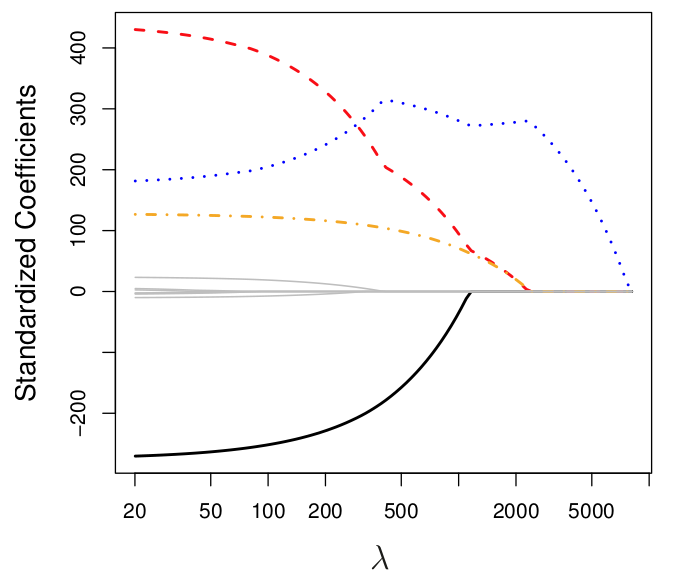
\includegraphics[width = \textwidth]{Fig6-6a}
	\column{.4\textwidth}
	\centering
	Ridge
	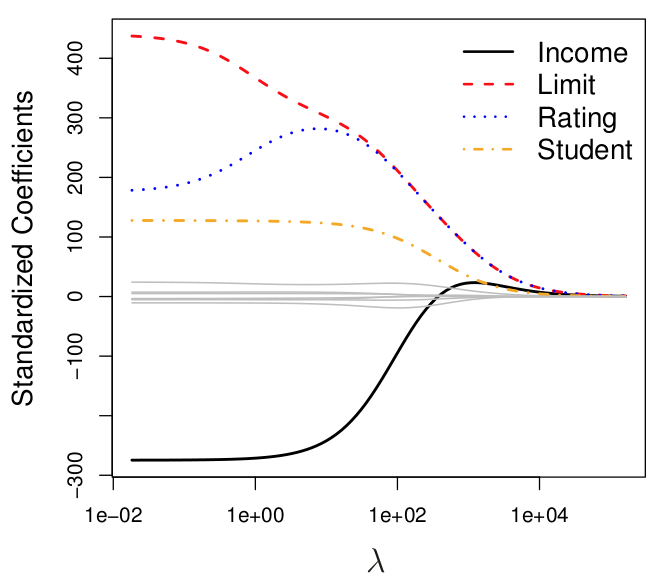
\includegraphics[width = \textwidth]{Fig6-4a}
	\end{columns}
	\InstructorList{
	\item $\lambda = 0$: Both are least squares
	\item $\lambda = \infty$: Everything is 0
	\item only lasso has 0 efficients at finite $\lambda$
	}
	
	\end{frame}

%--- Next Frame ---%
\begin{frame}[t]{Why the hell lasso can select variable (while ridge cannot)?}
	Alternative formulation of lasso \& ridge regression (\href{https://www.geogebra.org/graphing/euymx5b9}{play more with $\ell_p$})
	% \begin{columns}
	% 	\column{.4\textwidth}
		\begin{equation*}
			\min_\beta \sum (y_i-\hat{y}_i)^2 \text{ where } \sum |\beta_j|\leq s
		\end{equation*}
		\begin{equation*}
			\min_\beta \sum (y_i-\hat{y}_i)^2 \text{ where } \sum |\beta_j|^2\leq s
		\end{equation*}
	
		% -- picture
		% \column{.4\textwidth}
		\centering
		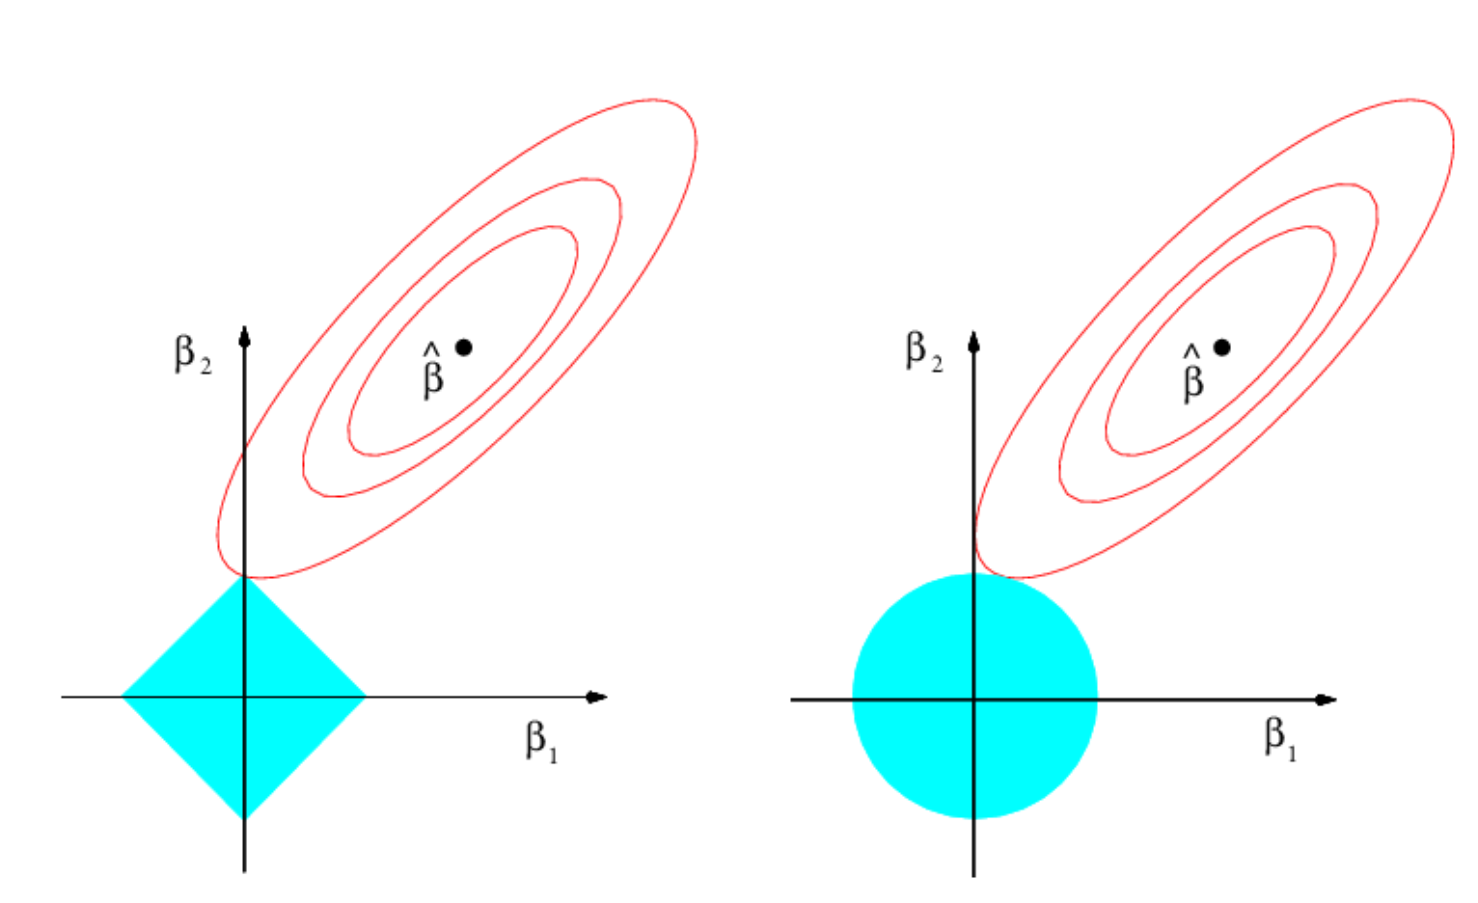
\includegraphics[width=0.5\textwidth]{lasso_ridge_contour.png}
	
	% \end{columns}
	\end{frame}

%--- Next Frame ---%

	\begin{frame}[t]{Subset selection example: best subset}
		We train a model using four variables, $X_1,X_2,X_3$.
		We're interested in getting a subset of the variables to use. The following table shows the training and test error for the model learned using each possible subset of variables.
		\begin{columns}
		\column{.45\textwidth}
		\centering
		% \begin{wrapfigure}{r}{1in}
		\begin{center}
		% 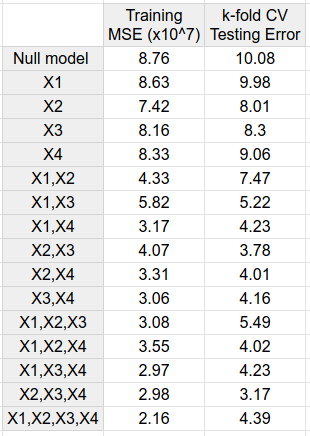
\includegraphics[width = .5\textwidth]{FakeData-SubsetSelection.png}
		\begin{tabular}{c | c | c}
				& Training MSE & K-fold CV test MSE\\
			\hline
			null model & 0.079 &	0.614\\
			\hline
			X1 &0.984	&0.954 \\
			\hline
			X2&0.172	&0.642\\
			\hline
			X3&0.410	&0.533\\
			\hline
			X1,X2&0.800	&0.810\\
			\hline
			X2,X3&0.696	&0.577\\
			\hline
			X1,X3&0.888	&0.779\\
			\hline
			X1,X2,X3&0.133	&0.536\\
			\hline
		\end{tabular}
		\end{center}
		% \end{wrapfigure}
		
		\column{.45\textwidth}
		\centering

		
		\end{columns}
		\end{frame}
% ---- next frame ---- %
\begin{frame}[t]{Subset selection example: forward selection}
	We train a model using four variables, $X_1,X_2,X_3$.
	We're interested in getting a subset of the variables to use. The following table shows the training and test error for the model learned using each possible subset of variables.
	\begin{columns}
	\column{.45\textwidth}
	\centering
	% \begin{wrapfigure}{r}{1in}
	\begin{center}
	% 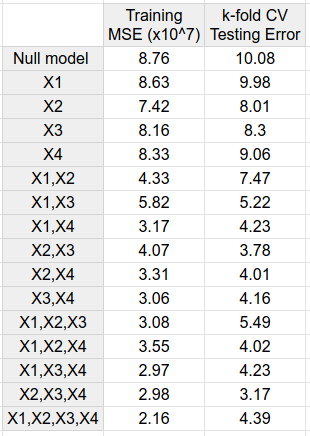
\includegraphics[width = .5\textwidth]{FakeData-SubsetSelection.png}
	\begin{tabular}{c | c | c}
			& Training MSE & K-fold CV test MSE\\
		\hline
		null model & 0.079 &	0.614\\
		\hline
		X1 &0.984	&0.954 \\
		\hline
		X2&0.172	&0.642\\
		\hline
		X3&0.410	&0.533\\
		\hline
		X1,X2&0.800	&0.810\\
		\hline
		X2,X3&0.696	&0.577\\
		\hline
		X1,X3&0.888	&0.779\\
		\hline
		X1,X2,X3&0.133	&0.536\\
		\hline
	\end{tabular}
	\end{center}
	% \end{wrapfigure}
	
	\column{.45\textwidth}
	\centering

	
	\end{columns}
	\end{frame}

	% ---- next frame ---- %
\begin{frame}[t]{Subset selection example: backward selection}
	We train a model using four variables, $X_1,X_2,X_3$.
	We're interested in getting a subset of the variables to use. The following table shows the training and test error for the model learned using each possible subset of variables.
	\begin{columns}
	\column{.45\textwidth}
	\centering
	% \begin{wrapfigure}{r}{1in}
	\begin{center}
	% 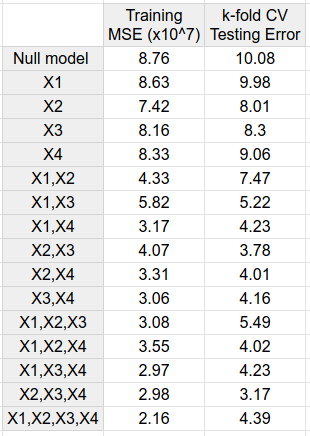
\includegraphics[width = .5\textwidth]{FakeData-SubsetSelection.png}
	\begin{tabular}{c | c | c}
			& Training MSE & K-fold CV test MSE\\
		\hline
		null model & 0.079 &	0.614\\
		\hline
		X1 &0.984	&0.954 \\
		\hline
		X2&0.172	&0.642\\
		\hline
		X3&0.410	&0.533\\
		\hline
		X1,X2&0.800	&0.810\\
		\hline
		X2,X3&0.696	&0.577\\
		\hline
		X1,X3&0.888	&0.779\\
		\hline
		X1,X2,X3&0.133	&0.536\\
		\hline
	\end{tabular}
	\end{center}
	% \end{wrapfigure}
	
	\column{.45\textwidth}
	\centering

	
	\end{columns}
	\end{frame}
\end{document}
